\documentclass{article}
\usepackage[utf8]{inputenc}

\usepackage{tikz}
\usetikzlibrary{positioning, fit}

\begin{document}

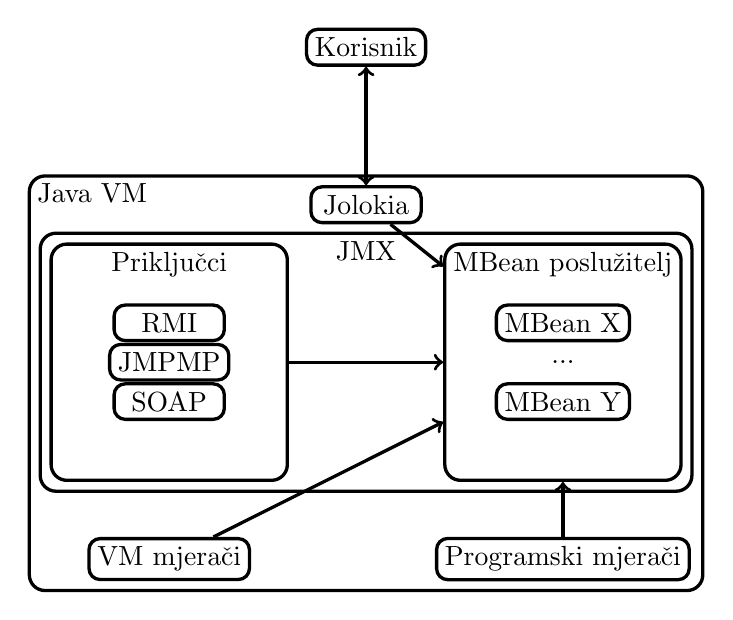
\begin{tikzpicture}[ % has a lot of options; consult the pgf manual
bend angle=15,
long_square/.style={rectangle, draw=black, fill=white, very thick, inner sep=3pt, minimum width=14mm},
rounded_square/.style={rectangle, rounded corners, draw=black, fill=white, very thick, inner sep=3pt, minimum width=14mm},
empty_circle/.style={rectangle, rounded corners=2mm, draw=black, fill=white, very thick, minimum size=4mm},
point/.style={circle, inner sep=0mm},
fit_square/.style={rectangle, rounded corners=2mm, draw=black, very thick, minimum height=30mm, minimum width=30mm},
both_arrow/.style={<->, very thick},
out_arrow/.style={->, very thick},
in_arrow/.style={<-, very thick},
above_edge_text/.style={above, midway, sloped}
]

\node[rounded_square](client) at (2.5,0) {Korisnik};

\node[rounded_square](jolokia) at (2.5,-2) {Jolokia};

\node[rounded_square](rmi) at (0,-3.5) {RMI};
\node[rounded_square](jmxmp) at (0,-4) {JMPMP};
\node[rounded_square](soap) at (0,-4.5) {SOAP};

\node[rounded_square](mbean_1) at (5,-3.5) {MBean X};
\node[](mbean_2) at (5,-4) {...};
\node[rounded_square](mbean_3) at (5,-4.5) {MBean Y};

\node[rounded_square](vm_instremuntation) at (0,-6.5) {VM mjerači};
\node[rounded_square](app_instremuntation) at (5,-6.5) {Programski mjerači};

\node[fit_square, fit=(rmi) (jmxmp) (soap)] (connectors) {};
\node[anchor=north] at (connectors.north) {Priključci};

\node[fit_square, fit=(mbean_1) (mbean_2) (mbean_3)] (server) {};
\node[anchor=north] at (server.north) {MBean poslužitelj};

\node[fit_square, fit=(connectors) (server)] (jmx) {};
\node[anchor=north] at (jmx.north) {JMX};

\node[fit_square, fit=(jmx) (vm_instremuntation) (app_instremuntation) (jolokia)] (java_vm) {};
\node[anchor=north west] at (java_vm.north west) {Java VM};



\draw[both_arrow](client) to [] node[auto]{} (jolokia);

\draw[out_arrow](jolokia) to [] node[auto]{} (server);

\draw[out_arrow](connectors) to [] node[auto]{} (server);

\draw[out_arrow](vm_instremuntation) to [] node[auto]{} (server);
\draw[out_arrow](app_instremuntation) to [] node[auto]{} (server);

\end{tikzpicture}

\end{document}